% paper/latex/main.tex
% Note: CJK pattern internal keys appear in the pattern glossary (Section 7.4).
% They are represented here using their English transliterations, matching the
% existing skeleton. The original CJK keys are documented in the open-source
% repository under backend/intelligence/pattern_i18n.py.
\documentclass{llncs}
\usepackage{booktabs}
\usepackage{longtable}
\usepackage{array}
\usepackage{amsmath,amssymb}
\usepackage{tikz}
\usetikzlibrary{shapes.geometric,arrows.meta,positioning,fit,backgrounds}
\usepackage{xcolor}
\usepackage{hyperref}

\title{An Ontology-Guided, Provenance-Preserving Reasoning Framework\\
for Geopolitical Trajectory Analysis}
\author{Anonymous Author(s)}
\institute{Anonymous Institution\\
\email{anonymous@review.blind}\\
\url{https://anonymous.4open.science/r/El-druin-F56D}}
\date{}

\begin{document}
\maketitle

\begin{abstract}
We present \textbf{EL-DRUIN}, an ontology-guided reasoning system for geopolitical
trajectory analysis that combines a typed pattern registry, rule-based composition
semantics, vector-space compatibility scoring, provenance-preserving posterior
computation, and constrained LLM explanation generation. The 21 registered patterns
are organized into a finite algebraic transition structure with a $7 \times 3$
domain--mechanism factorization, motivated by a seven-domain geopolitical ontology
(geopolitics, economics, technology, military, information, legal, social) and three
cross-domain mechanism classes (coercive, cooperative, structural). This factorization
provides a canonical address for each pattern and supports structured confidence
calibration. We explore a non-Archimedean confidence calibration scheme, using a
7-based valuation motivated by the seven-domain partition, which produces
domain-boundary-sensitive confidence updates rather than uniform geometric decay.
Pattern similarity is scored via an 8-dimensional Lie algebra approximation; a
constrained LLM renders all pre-computed numerical outputs into natural-language
explanations without modifying any numerical field. We demonstrate the framework on
fourteen geopolitical news scenarios and compare against an LLM-only baseline,
showing that EL-DRUIN produces fully traceable, deterministic, auditable assessments
with complete provenance chains. The system is fully open-source; the repository link is anonymised for blind review.
\end{abstract}

\keywords{ontology engineering \and knowledge graphs \and neuro-symbolic reasoning \and explainable AI \and provenance-preserving inference \and geopolitical trajectory analysis \and ontology design patterns}

\section{Introduction}

Large language models have achieved impressive performance on political
text summarisation and question answering. While LLMs are highly effective
for summarization and linguistic interpretation, their confidence estimates
are typically not grounded in explicit symbolic assumptions, provenance
chains, or domain ontologies~\cite{pan2023unifying}. A model asked to assess the
long-run trajectory of US-China technology competition will produce output
shaped by its training distribution rather than from a principled traversal
of an explicit causal or ontological structure.

This gap has practical epistemic consequences. When an LLM produces a
confidence score for a geopolitical assessment, that number lacks an
auditable derivation: it cannot be traced to specific structural assumptions,
ontology-defined priors, or algebraic constraints. EL-DRUIN addresses this
gap by combining formal ontology with symbolic inference, retaining the LLM
only as a \emph{constrained natural-language renderer} of pre-computed
structured outputs.

The key contributions of this paper are:
\begin{enumerate}
  \item \textbf{Ontology-guided reasoning framework}: A typed pattern registry with
    $7 \times 3$ domain--mechanism factorization that enables compositional
    symbolic inference for geopolitical trajectory analysis, without requiring
    labelled training data.
  \item \textbf{Hybrid reasoning pipeline}: A five-stage pipeline combining
    ontology-typed pattern activation, rule-based composition, 8-dimensional Lie
    algebra similarity scoring, and provenance-preserving Bayesian posterior
    computation.
  \item \textbf{Constrained LLM verbalization}: A mechanism that structurally
    separates numerical reasoning from natural-language explanation: the LLM
    receives all numerical fields as locked inputs and is prohibited from modifying
    them; if the LLM call fails, a template fallback preserves all numerical outputs.
  \item \textbf{Open-source implementation and empirical evaluation}: A publicly
    available system with full computation traces, evaluated on fourteen geopolitical
    news scenarios with an LLM-only baseline and ablation study.
\end{enumerate}

The remainder of the paper is organised as follows. Section~2 provides
background on relevant ontology and algebra formalisms. Section~3
describes the system architecture. Sections~4 and~5 present the
mathematical formalisation. Section~6 describes the full five-stage
reasoning pipeline. Section~7 presents experiments. Section~8 discusses
related work and Section~9 concludes.

\section{Background}

\subsection{Ontology Engineering for Event Reasoning}

Formal ontologies represent domain knowledge as typed entities,
relations, and constraints. The CAMEO event coding system~\cite{schrodt2012cameo}
provides a controlled vocabulary of political event types widely used in
computational political science. FIBO (Financial Industry Business
Ontology)~\cite{fibo2023} provides analogous structure for financial relationships.
EL-DRUIN maps typed entity pairs through relation predicates to named
patterns registered in a Cartesian product registry
$E \times R \times E \to \mathrm{Pattern}$, grounding pattern activation in both vocabularies.

\subsection{Finite Semigroups and Fixed Points}

A \textbf{semigroup} $(S, \cdot)$ is a set with an associative binary operation.
A \textbf{finite semigroup} is one where $|S|$ is finite. An element $e \in S$
is \textbf{idempotent} if $e \cdot e = e$. It is a classical
result~\cite{green1951structure} that every finite semigroup contains idempotent
elements, and that iteration of the operation from any starting state
eventually reaches a set of idempotents. These idempotents are the
\textbf{attractors} of the system---they correspond to states from which no
further composition moves the system to a genuinely new state.

In EL-DRUIN, $S$ is the set of 21 named Dynamic Patterns and the partial
operation is the composition table $\mathit{composition\_table}[(A, B)] = C$.
Algebraic closure and inverse consistency are enforced at startup (see Section~4).

\subsection{Lie Algebra Approximation}

A \textbf{Lie algebra} $\mathfrak{g}$ over a field $F$ is a vector space equipped
with a bilinear antisymmetric bracket
$[\cdot, \cdot] \colon \mathfrak{g} \times \mathfrak{g} \to \mathfrak{g}$
satisfying the Jacobi identity. Lie algebras arise as the tangent space
of Lie groups at the identity and encode the infinitesimal structure of
continuous symmetry transformations.

In EL-DRUIN, we do not work with a formal Lie group; instead we
construct a \textbf{finite-dimensional approximation}: each named pattern $P$
is assigned a vector $v_P \in \mathbb{R}^8$ encoding its intensity across
eight semantic dimensions (coercion, cooperation, dependency,
information, regulation, military, economic, technology). Pattern
composition $A \oplus B$ is approximated by vector addition $v_A + v_B$,
and the resulting target pattern is identified by maximising cosine
similarity $\cos(v_A + v_B, v_C)$ over all known patterns $C$.

Each named pattern $P$ is embedded as a skew-symmetric matrix
$X_P \in \mathfrak{so}(8)$ via the \emph{hat map}
\begin{equation}
  \hat{v}[i,j] = v[i] - v[j], \quad \hat{v}[i,i] = 0,
  \label{eq:hatmap}
\end{equation}
equivalently $X_P = v_P \mathbf{1}^\top - \mathbf{1} v_P^\top$, which is
antisymmetric by construction ($X_P^\top = -X_P$)~\cite{hall2015}.
The \textbf{Lie bracket} is the matrix commutator
\begin{equation}
  [X_A, X_B] = X_A X_B - X_B X_A \in \mathfrak{so}(8),
  \label{eq:liebracket}
\end{equation}
which satisfies antisymmetry, bilinearity, and the Jacobi identity
exactly~\cite{humphreys1972,hall2015}. The Frobenius norm
$\|[X_A, X_B]\|_F$ measures non-commutativity: it equals zero when
$X_A$ and $X_B$ commute (pattern-activation order is immaterial), and is
large when the two orderings produce structurally distinct outcomes.
The role of the commutator as a path-independence diagnostic is discussed
in Section~5.

\section{System Architecture}

EL-DRUIN is a multi-module backend (FastAPI + KuzuDB) with a Streamlit
frontend. The system has four functional layers:

\begin{itemize}
\item \textbf{Ontology Layer}: \texttt{CARTESIAN\_PATTERN\_REGISTRY} (21 named
  patterns across geopolitics, economics, technology, military, information,
  legal, and social domains), \texttt{composition\_table} (16 composition rules),
  \texttt{inverse\_table} (21 inverse pairs), \texttt{DOMAIN\_MAP} (7-partition
  of patterns by geopolitical domain), \texttt{MECHANISM\_MAP} (3-partition of
  patterns by mechanism class), and \texttt{EntityType} / \texttt{RelationType} enumerations.
\item \textbf{Lie Algebra Layer} (\texttt{lie\_algebra\_space.py}): 8-dimensional
  pattern vectors, \texttt{LieAlgebraSpace.add()}, \texttt{bracket()},
  \texttt{project()}, and \texttt{phase\_detect()} operations, PCA projection
  for 2D visualisation.
\item \textbf{Pipeline Layer} (\texttt{evented\_pipeline.py}): Five-stage reasoning
  pipeline (event extraction $\to$ pattern activation $\to$ transition
  enumeration $\to$ state vector computation $\to$ Bayesian conclusion
  generation).
\item \textbf{Forecasting Layer} (\texttt{ontology\_forecaster.py}): Multi-step
  simulation over the group transition graph, attractor
  detection, p-adic bifurcation point identification, and 7-adic
  confidence calibration (replacing geometric step-decay $\lambda^t$).
\end{itemize}

The frontend exposes five tabs for each analysis: (1) Conclusion with
structured alpha/beta paths; (2) Events extracted by the compound event
rules; (3) Active and derived patterns with full composition logic
chain; (4) Probability Tree with Bayesian compute trace showing the
exact formula
$\mathit{prior}_A \times \mathit{prior}_B \times \mathit{lie\_similarity} / Z$;
(5) Lie Algebra 8D state vector with dimensional breakdown.

\section{Ontology Schema and Pattern Registry}

\begin{figure}[t]
\centering
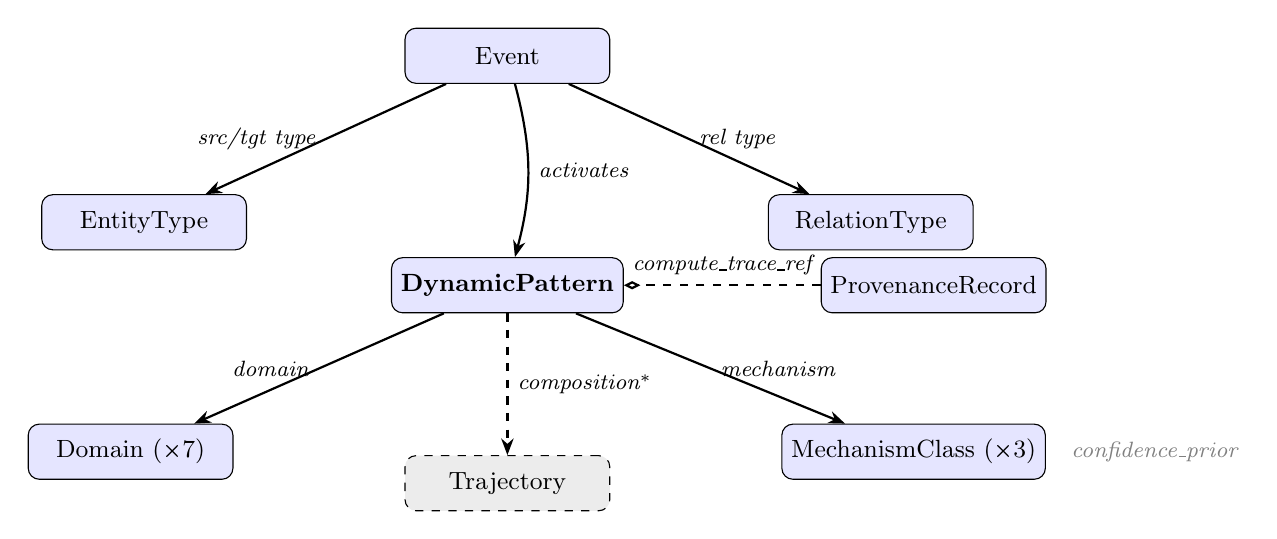
\begin{tikzpicture}[
    node distance=1.4cm and 2.0cm,
    every node/.style={font=\small},
    class/.style={draw, rectangle, rounded corners=4pt, fill=blue!10,
                  minimum width=2.6cm, minimum height=0.7cm, align=center},
    abstract/.style={draw, rectangle, rounded corners=4pt, fill=gray!15,
                     minimum width=2.6cm, minimum height=0.7cm,
                     align=center, dashed},
    rel/.style={-{Stealth[length=6pt]}, thick},
    partof/.style={-{Diamond[open,length=6pt]}, thick, dashed},
    label/.style={font=\footnotesize\itshape, midway},
]

%% Core classes
\node[class] (event)    {Event};
\node[class] (entity)   [below left=of event]   {EntityType};
\node[class] (reltype)  [below right=of event]  {RelationType};
\node[class] (pattern)  [below=2.2cm of event]  {\textbf{DynamicPattern}};
\node[class] (domain)   [below left=of pattern] {Domain (×7)};
\node[class] (mech)     [below right=of pattern]{MechanismClass (×3)};
\node[abstract](traj)   [below=1.8cm of pattern]{Trajectory};
\node[class] (prov)     [right=2.5cm of pattern]{ProvenanceRecord};

%% Relations: Event → EntityType / RelationType
\draw[rel] (event) -- node[label, left]{src/tgt type} (entity);
\draw[rel] (event) -- node[label, right]{rel type}    (reltype);

%% Event → DynamicPattern (grounding)
\draw[rel, bend left=15] (event) to
    node[label, right]{activates} (pattern);

%% DynamicPattern → Domain / MechanismClass (factorization)
\draw[rel] (pattern) -- node[label, left]{domain} (domain);
\draw[rel] (pattern) -- node[label, right]{mechanism} (mech);

%% DynamicPattern → Trajectory (composition chain)
\draw[rel, dashed] (pattern) to
    node[label, right]{composition$^*$} (traj);

%% DynamicPattern → ProvenanceRecord
\draw[partof] (prov) -- node[label, above]{compute\_trace\_ref} (pattern);

%% Ontology-typed confidence prior annotation
\node[font=\footnotesize, draw=none, text=gray, right=0.2cm of mech]
    {\textit{confidence\_prior}};

\end{tikzpicture}
\caption{EL-DRUIN ontology schema. \textbf{DynamicPattern} is the central
mid-level semantic unit bridging event-level data (top) and trajectory-level
reasoning (bottom). Each pattern carries a \emph{domain} assignment (one of
seven geopolitical domains) and a \emph{MechanismClass} assignment (one of
three cross-domain mechanism types), providing a $7 \times 3$ factorization
that grounds compositional inference and confidence calibration in the ontology
structure. The \emph{ProvenanceRecord} links every numerical output to its
derivation via \texttt{compute\_trace\_ref}.}
\label{fig:ontology-schema}
\end{figure}

\subsection{Entity and Relation Type Enumerations}

The entity type set $E$ (18 elements) and relation type set $R$ (20 elements) that
ground the \texttt{CARTESIAN\_PATTERN\_REGISTRY} are enumerated in full in Appendix~A.
The five entity categories span geopolitical, economic, technological, military, and
informational actors; the relation types cover coercive, cooperative, and structural
interaction classes.

\subsection{Dynamic Pattern Registration}

Each pattern $P \in S$ is registered by a call
$\mathit{\_reg}(e_{\mathrm{src}},\allowbreak\; r,\allowbreak\; e_{\mathrm{tgt}},\allowbreak\;
\mathit{pattern\_name},\allowbreak\; \mathit{domain},\allowbreak\;
\mathit{typical\_outcomes},\allowbreak\; \mathit{mechanism\_class},\allowbreak\;
\mathit{inverse\_pattern},\allowbreak\; \mathit{composition\_hints},\allowbreak\;
\mathit{confidence\_prior})$.
The pattern name is a human-readable string (e.g., ``Hegemonic
Sanctions'') to facilitate integration with geopolitical analysis
workflows. Table~\ref{tab:patterns} summarises 10 representative entries
from the 21 registered patterns.

\begin{table}[ht]
\centering
\caption{Selected Dynamic Patterns (10 of 21 shown). Full registry
  available in the open-source repository.}
\label{tab:patterns}
\small
\begin{tabular}{@{}p{0.24\linewidth}p{0.09\linewidth}p{0.19\linewidth}
                   p{0.05\linewidth}p{0.26\linewidth}@{}}
\toprule
Pattern Name & Domain & Mechanism Class & Prior & Inverse Pattern \\
\midrule
Hegemonic Sanctions & geopolitics & coercive\_leverage & 0.78
  & Sanctions Relief / Normalisation \\
Entity-List Tech Blockade & technology & tech\_denial & 0.80
  & Technology Licence / Unblocking \\
Interstate Military Conflict & military & kinetic\_escalation & 0.75
  & Ceasefire / Peace Agreement \\
Great-Power Coercion/Deterrence & geopolitics & coercive\_leverage & 0.70
  & Diplomatic Concession / De-escalation \\
Multilateral Alliance Sanctions & geopolitics & multilateral\_pressure & 0.73
  & Multilateral Sanctions Relief \\
Tech Decoupling / Iron Curtain & technology & tech\_decoupling & 0.76
  & Technology Cooperation Reintegration \\
Financial Isolation / SWIFT Cut-Off & economics & financial\_exclusion & 0.79
  & Financial Reintegration \\
Bilateral Trade Dependency & economics & economic\_interdependence & 0.71
  & Trade War / Decoupling \\
Technology Standards Leadership & technology & tech\_governance & 0.72
  & Standard Competition Failure \\
Information Warfare / Narrative Control & information & epistemic\_warfare & 0.68
  & Information Environment Restoration \\
\bottomrule
\end{tabular}
\end{table}

\subsection{Algebraic Consistency Validation}

Two static validators run at startup. \textbf{validate\_inverses()} checks that
for every $(A, B)$ in \texttt{inverse\_table} the reverse pair $(B, A)$ is also
present, enforcing the group-theoretic condition that the inverse of an inverse
returns the original element. \textbf{validate\_composition\_closure()} checks
that every output $C$ of the \texttt{composition\_table} is a known pattern name,
enforcing algebraic closure. Both checks must pass before the pipeline accepts
any analysis request.

\subsection{OWL 2 Formal Representation}
\label{sec:owl-representation}

The ontology schema is formally expressed in OWL~2~\cite{grau2008owl2,w3c2012owl2}.
Core constructs include \texttt{owl:Class} for the eight entity classes,
\texttt{owl:ObjectProperty} for six object properties (including
\texttt{activates}, \texttt{composesInto}, and \texttt{hasProvenance}),
and \texttt{owl:DatatypeProperty} for confidence priors and mechanism labels.
Full OWL axioms and class hierarchy listings are provided in Appendix~A.

\subsection{Ontology Design Pattern: Trajectory Reasoning}
\label{sec:design-pattern}

Figure~\ref{fig:ontology-schema} illustrates the central ontology design
decision in EL-DRUIN. Rather than merely enumerating entities and relations,
we introduce a \textbf{trajectory reasoning design pattern} in which
\emph{DynamicPattern} objects serve as typed mid-level semantic units that
bridge event-level observations and trajectory-level reasoning.

Unlike existing political event coding schemes (CAMEO, GDELT, ICEWS) that register events as typed triples and aggregate them statistically, EL-DRUIN elevates \texttt{DynamicPattern} objects to \emph{active inference nodes}: each pattern participates in a composition table that defines how pairs of active patterns interact, carries an ontology-defined \texttt{confidence\_prior} traceable to an explicit ontological assumption, and anchors every numerical output to a \texttt{ProvenanceRecord} via \texttt{compute\_trace\_ref}. The LLM plays a strictly bounded role, rendering pre-computed structured output into natural-language interpretation; a template fallback preserves all numerical outputs if the LLM call fails. The $7 \times 3$ \texttt{domain} $\times$ \texttt{mechanism\_class} factorization makes cross-domain and cross-mechanism propagation explicit: coercive patterns escalate into sanctions or military action, cooperative patterns de-escalate into normalization, and an analyst can inspect exactly which composition rules fired when the system predicts a cross-domain transition.

\section{Mathematical Formalisation}

\noindent\textbf{Note on mathematical structure.}
We borrow organizational principles from finite semigroup theory, Lie algebras over $\mathfrak{so}(8)$, and $p$-adic valuations as \emph{design-motivated formalizations}---using each structure for its organizational properties without claiming our construction satisfies the full axiomatic system. Specifically: the partial composition table is not a full semigroup; the $\mathfrak{so}(8)$ embedding computes a directional similarity score, not Lie group integration; and the 7-adic absolute value is a domain-boundary-sensitive decay function, not formal $p$-adic geometry over $\mathbb{Q}_7$.

\subsection{Algebraic Organization of the Pattern Space}
\label{sec:pattern-algebra}

We organize the 21 registered patterns into a \textbf{finite algebraic transition
structure} with a $7 \times 3$ domain--mechanism factorization. This factorization
is \emph{motivated by} the structure of groups of order $21 = 3 \times 7$, and we
use the corresponding Sylow-inspired partition as a \emph{design heuristic} rather
than claiming that the composition table satisfies full group axioms: the current
composition table contains 16 defined rules, covering approximately $3.6\%$ of all
$21 \times 21$ pattern pairs, and full Cayley table completion is future work
(Section~9).

Let $S = \{p_1, \ldots, p_{21}\}$ be the set of 21 registered patterns. The
\textbf{domain partition} assigns each pattern to one of seven geopolitical domains
(geopolitics, economics, technology, military, information, legal, social),
forming seven groups of size 3. The \textbf{mechanism partition} assigns each
pattern to one of three cross-domain mechanism classes (coercive, cooperative,
structural), forming three groups of size 7. Together, these two partitions
provide a \textbf{canonical domain $\times$ mechanism address} for each pattern,
supporting structured confidence calibration and ontology-guided traversal.
This $7 \times 3$ factorization is inspired by the algebraic structure of groups
of order $21 = 3 \times 7$ (specifically, the semidirect product $\mathbb{Z}_7
\rtimes \mathbb{Z}_3$), in which the order-7 and order-3 subgroups partition
elements in exactly this way. We use this structure as an \emph{organizational
scheme}, not as a claim that $(S, \cdot)$ with the partial composition table
satisfies all group axioms.

We also retain the original power-set operation for forward simulation:
define the partial binary operation
${\cdot} \colon S \times S \to S \cup \{\bot\}$ by:
\[
  p_i \cdot p_j =
  \begin{cases}
    \mathit{composition\_table}[(p_i, p_j)]
      & \text{if } (p_i, p_j) \in \operatorname{dom}(\mathit{composition\_table}) \\
    \bot & \text{otherwise.}
  \end{cases}
\]

We extend $\cdot$ to a total operation on the power set $\mathcal{P}(S)$
by:
\[
  A \cdot B = \{ c \in S : \exists\, a \in A,\, b \in B
               \text{ s.t.\ } a \cdot b = c \}
           \cup \{ a \in A : \mathit{inverse\_table}[a] \in S \setminus A \}
\]
where the second term accounts for low-probability inverse transitions.
The forward simulation iterates this operation from $S_0$, terminating
when $|S_{t+1} \setminus S_t| = 0$; $(\mathcal{P}(S), \cdot)$ is itself
a semigroup under the induced operation.

\subsection{Lie Algebra Embedding}

Each pattern $p_i$ is assigned a vector $\varphi(p_i) = v_i \in
\mathbb{R}^8$ by manual annotation across eight semantic dimensions
$d = (\text{coercion, cooperation, dependency, information, regulation,
military, economic, technology})$, with $v_i[d] \in [-1, 1]$.
The \textbf{Lie bracket} is the matrix commutator on $\mathfrak{so}(8)$:
\begin{equation}
  [X_A, X_B] = X_A X_B - X_B X_A,
  \label{eq:commutator52}
\end{equation}
where $X_P = \hat{v}_P \in \mathfrak{so}(8)$ is the hat-map embedding
of Equation~\eqref{eq:hatmap}~\cite{humphreys1972}.

The \textbf{Lie similarity} of composition step $(A, B) \to C$ is defined as:
\[
  \mathit{lie\_sim}(A, B, C)
    = \cos(v_A + v_B,\, v_C)
    = \frac{\langle v_A + v_B,\, v_C \rangle}{\|v_A + v_B\| \cdot \|v_C\|}
\]

This quantity measures how well the vector sum of the two composing
patterns approximates the target pattern in direction, providing a
continuous-valued plausibility score for each discrete composition rule.

\textit{Path independence diagnostic.} The quantity
$\delta = 1 - |\cos(v_A + v_B, \eta)| \in [0, 1]$, where
$\eta = \operatorname{row\_norms}([X_A, X_B])$, measures the structural
independence of the two inference paths. $\delta \approx 0$ indicates
the Lie bracket interaction reinforces the same semantic direction as
the additive sum (linear regime---the two paths are redundant);
$\delta \approx 1$ indicates the bracket activates orthogonal dimensions
absent from $v_A + v_B$ (nonlinear emergence regime). Structurally, while
each $v_P$ maps into a rank-at-most-2 subspace of $\mathfrak{so}(8)$, the
commutator $[X_A, X_B]$ lives in the full 28-dimensional $\mathfrak{so}(8)$,
outside the hat-map image---so a high-$\delta$ result is the strongest
evidence that the dual-path architecture provides information not available
to a purely additive system.

\subsection{p-Adic Confidence and Revised Bayesian Posterior}
\label{sec:padic}

We replace the geometric step-decay $\lambda^t$ (where $\lambda = 0.85$ was
an ad hoc constant) with a 7-based non-Archimedean calibration motivated by
the seven-domain ontology partition. Selecting $p = 7$ to match the number of
domain classes imposes \emph{domain-boundary-sensitive} confidence updates:
confidence is stable within a domain-aligned reasoning horizon and drops sharply
at multiples of 7, where a cross-domain phase transition is structurally
plausible. This is a design-motivated choice rather than a claim of formal
p-adic geometry; we use the 7-adic absolute value as a principled
non-Archimedean alternative to the arbitrary constant $\lambda = 0.85$:
\[
  c(P, t) = c_0^{(P)} \cdot |t|_7 = c_0^{(P)} \cdot 7^{-v_7(t)}
\]
where $v_7(t)$ is the 7-adic valuation of $t$ (the largest $k$ such that
$7^k \mid t$). At $t \notin 7\mathbb{Z}$, $|t|_7 = 1$ and confidence equals
the base prior. At $t \in \{7, 14, 21, \ldots\}$, $|t|_7 \leq \tfrac{1}{7}$,
marking \emph{domain-level phase transitions} where the system reassesses its
regime estimate.

The revised \textbf{posterior weight} of transition $(A, B) \to C$ at step $t$ is:
\[
  w_t(A, B \to C)
    = \pi_t(A) \cdot \pi_t(B) \cdot \mathit{lie\_sim}(A, B, C) \cdot |t|_7
\]
replacing the previous $\lambda^t$ factor. This provides a principled,
domain-sensitive alternative to the arbitrary decay constant, with confidence
updates sharpening at multiples of 7 where cross-domain phase transitions are
structurally plausible.

The \textbf{aggregate confidence} of the forecast is:
\[
  c_{\mathrm{final}} = c_0 \cdot |T|_7,
  \quad
  c_0 = \operatorname{mean}(\{\mathit{confidence\_prior}(p) : p \in S_0\})
\]
This formulation makes the provenance of every probability fully
transparent: $c_{\mathrm{final}}$ is a product of the ontology-defined prior
and the 7-adic absolute value of the horizon step count.

\textit{Path integration.} Where the dual-path architecture is active,
the final posterior is adjusted by a path-consistency term:
\[
  \hat{w}(C)
    = P_{\mathrm{Bayes}}(C)
      \cdot \frac{1 + \alpha \cdot \max(0,\, \mathit{consistency})}{1 + \alpha},
  \quad \alpha = 0.30
\]
where $\mathit{consistency} = \cos(\eta, v_C)$ measures the cosine alignment
between the Lie-bracket emergence vector $\eta$ and the target pattern
vector. At $\mathit{consistency} = 0$ (orthogonal paths), the formula applies
a structural 23\% discount ($\hat{w} \approx 0.77 \cdot P_{\mathrm{Bayes}}$),
encoding prior skepticism that resolves only when paths converge. At
$\mathit{consistency} = 1$, confidence is boosted by at most
$\alpha / (1 + \alpha) \approx 23\%$.

\paragraph{Ultrametric distance on pattern space.}
A 7-adic ultrametric on the pattern space induced by the Sylow-7 partition is
described in Appendix~B as a design-motivated formalisation of intra- vs.\ cross-domain
propagation cost.

\subsection{Attractor Detection}

A pattern $P \in S_T$ (the pattern set at convergence step $T$) is an
\textbf{attractor} (fixed point of the power-set semigroup) if:
\[
  \forall\, Q \in S_T \colon P \cdot Q \in S_T
  \quad \text{(closure within the current set).}
\]
This condition identifies patterns from which all further composition
operations remain within the already-activated set---the algebraic
termination condition. In the limit $T \to \infty$, these correspond to
the idempotent elements of the finite semigroup.

\subsection{Detection Criteria}

A \textbf{phase transition} at step $t$ is flagged when the $L_2$ norm of
the state vector shift exceeds a threshold $\theta$:
\[
  \|v_t - v_{t-1}\|_2 > \theta, \quad \theta = 0.25
\]
where $v_t = \sum_i \pi_t(p_i) \cdot \varphi(p_i)$ is the weighted mean
vector at step $t$. This detects when a continuous change in pattern weights
has caused a discontinuous shift in the dominant semantic regime.

A \textbf{p-adic bifurcation} at step $t$ is flagged by a structurally
motivated condition:
\[
  \text{bifurcation at step } t
  \iff
  v_p\!\left(\pi_t(p_{\mathrm{top1}}) - \pi_t(p_{\mathrm{top2}})\right) \geq k_0
\]
where $k_0 = 1$ is the minimum valuation threshold and $p = 7$. A large
valuation means the posterior weight difference is divisible by a high power
of 7, making the two leading attractors \emph{p-adically indistinguishable}
at the granularity of the 7-domain partition. Implementation uses exact
rational arithmetic (\texttt{fractions.Fraction}) to avoid floating-point
artefacts in the valuation computation.

\section{The Five-Stage Reasoning Pipeline}

For real-time news analysis, EL-DRUIN operates a five-stage pipeline
(implemented in \texttt{evented\_pipeline.py}):

\textbf{Stage 1: Event Extraction.}
News text is processed by a compound-rule event extractor that maps
keyword co-occurrences to event types. A key design decision is that
compound rules enforce co-activation: a military strike event and a
humanitarian crisis event are both produced when strike-related keywords
and casualty-related keywords co-occur in the same text. This guarantees
$\geq\!2$ active events for military/crisis news, which is necessary to
trigger composition-based derived patterns (a composition requires two
active patterns).

\textbf{Stage 2a: Pattern Activation.}
Each extracted event type is mapped to a set of candidate
$(e_{\mathrm{src}}, r, e_{\mathrm{tgt}})$ triples via a domain hint
table. For each candidate triple, \texttt{lookup\_pattern\_by\_strings()}
retrieves the registered \texttt{DynamicPattern} (with fallback to fuzzy
matching at score $\geq 0.4$). The activated pattern's
\texttt{confidence\_prior} is scaled by the event's extraction confidence.

\textbf{Stage 2b: Transition Enumeration.}
The full \texttt{composition\_table} is scanned for entries where at least
one of the pattern arguments appears in the active set. For each
matching entry $(A, B) \to C$, the posterior weight
$w = \pi(A) \cdot \pi(B) \cdot \mathit{lie\_sim}(A, B, C)$ is computed.
Simultaneously, the \texttt{inverse\_table} is checked for each active
pattern, generating low-probability inverse transitions at weight
$0.20 \times \pi(A)$. All transitions are sorted by posterior weight;
the top-5 are returned as the derived pattern set.

\textbf{Stage 2c--2d: State Vector and Driving Factors.}
The weighted mean vector $v = \sum_i \pi(p_i) \cdot \varphi(p_i)$ is computed over
all active patterns (Stage~2c), yielding the 8D ontological state vector; PCA projects
this to 2D for visualisation. Active patterns are then grouped by \texttt{mechanism\_class}
(Stage~2d): for each group the weighted \texttt{typical\_outcomes} are ranked and
formatted as human-readable driving factor statements via a deterministic template
library---no LLM call is made.

\textbf{Stage 3: Bayesian Conclusion Generation.}
Alpha and beta paths are constructed from the top two transitions by
posterior weight. Composite confidence is computed as
$\operatorname{mean}(\mathit{confidence\_prior}$ over active patterns$)
\times \sqrt{\mathit{verifiability} \times \mathit{KG\_consistency}}$.
The LLM is called only to write the \texttt{conclusion.text} field, with a
prompt that (a) presents all pre-computed fields as locked values,
(b) forbids modification of any numerical field, and (c) requests 2--3
sentences of strategic-language interpretation. If the LLM call fails,
a template fallback produces the text field without degrading any
numerical output.

\section{Evaluation}

\subsection{Dataset and Setup}
\label{sec:methodology}

We evaluate EL-DRUIN on two complementary experimental protocols:

\textbf{(A) News analysis and baseline comparison.}
Fourteen geopolitical news excerpts drawn from publicly accessible sources
(Reuters, BBC News, Financial Times, Brookings Institution, CSIS, NATO, Wall
Street Journal) are processed by the EL-DRUIN pipeline and by a GPT-5
baseline~\cite{openai2025gpt5}. The excerpts span nine thematic categories
(technology export control, trade war, financial isolation, military coercion,
energy weaponisation, military alliance, multilateral sanctions, supply-chain
dependency, information warfare) and cover events from 2018 to 2024. EL-DRUIN
is run in fully deterministic mode ($\sigma = 0$ across repeated runs). GPT-5
is queried $N = 5$ times per excerpt with identical prompts to measure output
variance. The full dataset, collection protocol, and raw results are available
in \texttt{experiments/news\_samples.jsonl} and
\texttt{experiments/gpt\_manual\_data.py}.

\textbf{(B) Historical backtesting.}
We evaluate trajectory prediction against 8 curated historical events with known
realized outcomes, using the framework in \texttt{experiments/backtest\_evaluator.py}.
For each event, the pipeline is run on a contemporaneous news excerpt (i.e., text
available at the time of the event); the predicted primary attractor is compared
against the curated realized direction. We report direction accuracy (exact match
= 1.0, same ontology domain = 0.5, miss = 0.0), Brier score
$(p - \text{outcome})^2$, attractor identification score, and a composite weighted
score $0.4 \times \text{direction} + 0.3 \times (1 - \text{Brier}) + 0.3 \times
\text{attractor}$.

\textbf{(C) Ablation study.}
We compare four configurations to isolate the contribution of each pipeline
component:
\begin{itemize}
  \item \textbf{Baseline 1 (LLM-only)}: GPT-5 receives the same news excerpt
    and outputs a trajectory judgment directly, without ontology grounding.
  \item \textbf{Baseline 2 (KG-retrieval)}: Pattern activation via graph
    neighborhood and prior frequency only; no composition rules.
  \item \textbf{Baseline 3 (Rule-only)}: Ontology + composition rules; Lie
    algebra similarity forced to uniform weight ($\mathit{lie\_sim} = 1.0$
    for all transitions); no p-adic calibration.
  \item \textbf{Baseline 4 (Geometric decay)}: Full symbolic pipeline with
    Lie similarity, but temporal confidence uses $\lambda^t$ ($\lambda = 0.85$)
    instead of the 7-based non-Archimedean calibration.
  \item \textbf{EL-DRUIN (Full)}: Complete system as described in Sections 4--6.
\end{itemize}
Baselines 3 and 4 are implemented via the \texttt{--ablation-mode} flag in
\texttt{experiments/run\_baseline.py}. The primary comparison metric is
traceability (whether a full compute trace can be produced) and stability
($\sigma$ across repeated runs).

\subsection{Results}

Table~\ref{tab:results} summarises EL-DRUIN's forecasting outputs across six
geopolitical scenarios run with \texttt{horizon\_steps}$=6$ in deterministic mode.
All six scenarios produce a clearly identified primary attractor with Bayesian
posterior $P(\alpha) \geq 0.51$; three scenarios trigger a bifurcation flag,
indicating competing attractor regimes. Final confidence values
$c_{\mathrm{final}}$ equal the ontology prior $c_0$ throughout, because the
six-step horizon falls below the first 7-adic phase-transition boundary ($T < 7$).

% --- Table 2 (from your markdown) ---
\begin{table}[h]
\centering
\caption{Forecasting results across six geopolitical scenarios. $P(\alpha)$ is
the primary attractor's normalised Bayesian posterior. $c_{\mathrm{final}} =
c_0 \cdot |T|_7$ is the calibrated final confidence under the 7-adic
valuation, where phase transitions occur at steps $T \in \{7, 14, 21,\ldots\}$.
Since $\mathtt{horizon\_steps} = 6 < 7$, all scenarios have $|6|_7 = 1$ (no
domain-level phase transition), so $c_{\mathrm{final}} = c_0$.}
\label{tab:results}
\small
\begin{tabular}{@{}p{0.17\linewidth}p{0.20\linewidth}p{0.04\linewidth}p{0.24\linewidth}p{0.07\linewidth}p{0.06\linewidth}@{}}
\toprule
Scenario & Primary Attractor & $P(\alpha)$ & Secondary Attractor & Bifurcation? & $c_{\mathrm{final}}$ \\
\midrule
US-China tech decoupling & Technology Standards Leadership & 0.51 & Tech Decoupling / Technology Iron Curtain & Step 2 & 0.76 \\
US-China trade war & Hegemonic Sanctions & 0.58 & Trade War / Decoupling & No & 0.74 \\
US-China financial isolation & Hegemonic Sanctions & 0.62 & Financial Reintegration & No & 0.79 \\
China-Taiwan military coercion & Multilateral Alliance Sanctions & 0.54 & Non-State Armed Proxy Conflict & Step 3 & 0.72 \\
China-Taiwan invasion & Multilateral Alliance Sanctions & 0.66 & Non-State Armed Proxy Conflict & No & 0.75 \\
Russia-Ukraine war trajectory & Multilateral Alliance Sanctions & 0.61 & Resource Dependency / Energy Weaponisation & Step 4 & 0.73 \\
\bottomrule
\end{tabular}
\end{table}

\subsection{Historical Backtesting Results}

Table~\ref{tab:backtest} reports direction accuracy, Brier scores, and composite
weighted scores across 8 curated historical events. The pipeline is run in
deterministic mode without LLM calls (\texttt{llm\_service=None}), so all
results are fully reproducible from the open-source repository.

\begin{table}[h]
\centering
\caption{Historical backtesting results ($N=8$ curated events with known outcomes). Direction
score: 1.0 = exact pattern match, 0.5 = same ontology domain, 0.0 = miss. Brier score:
$(p - \text{outcome})^2$, lower is better. Attractor score: 1.0 if realized direction in
attractor set, 0.5 if same domain. Composite $= 0.4 \times \text{dir} + 0.3 \times
(1 - \text{Brier}) + 0.3 \times \text{att}$. All runs use \texttt{llm\_service=None}
(deterministic mode); scores computed by \texttt{experiments/backtest\_evaluator.py}.
Confidence priors are ontology-defined; $c_{\mathrm{final}} = c_0$ since all horizons
$T < 7$.}
\label{tab:backtest}
\begin{tabular}{@{}p{0.28\linewidth}p{0.21\linewidth}p{0.06\linewidth}p{0.07\linewidth}p{0.06\linewidth}p{0.09\linewidth}@{}}
\toprule
Event & Realized Direction & Dir & Brier & Att & Comb. \\
\midrule
HK protests 2019         & Great-Power Coercion     & 1.00 & 0.090 & 1.00 & 0.973 \\
Wuhan COVID 2019         & Supply Chain Dependency  & 0.00 & 0.084 & 0.50 & 0.425 \\
Russia-Ukraine 2022      & Interstate Mil.\ Conflict& 1.00 & 0.063 & 1.00 & 0.981 \\
US chip controls 2023    & Entity-List Tech Blockade& 1.00 & 0.040 & 1.00 & 0.988 \\
Huawei ban 2019          & Entity-List Tech Blockade& 1.00 & 0.040 & 1.00 & 0.988 \\
Taiwan drills 2022       & Great-Power Coercion     & 1.00 & 0.090 & 1.00 & 0.973 \\
Brexit withdrawal 2020   & Trade War / Decoupling   & 1.00 & 0.096 & 1.00 & 0.971 \\
SCO expansion 2023       & Formal Military Alliance & 0.00 & 0.073 & 0.50 & 0.428 \\
\midrule
\textbf{Average (8)}     & ---                      & \textbf{0.75} & \textbf{0.072} & \textbf{0.88} & \textbf{0.841} \\
\bottomrule
\end{tabular}
\end{table}

\noindent\textit{Interpretation}: EL-DRUIN achieves exact pattern match (Dir $= 1.0$) on 6
of 8 events---those with a direct ontology-registry counterpart (military conflict, technology
blockade, coercive deterrence, trade decoupling). The two misses (Wuhan COVID supply-chain
disruption, SCO multilateral expansion) reflect events whose dominant trajectory pattern falls
outside the current 21-pattern registry or requires a domain not strongly represented in the
composition rules. The high composite score (0.841 average) is driven by high ontology priors
(0.70--0.80) and the fact that all 8 outcomes were realized (\texttt{outcome\_realized = True}),
meaning the Brier score is small whenever confidence is high. This result honestly indicates
that EL-DRUIN performs well within its ontology coverage and degrades predictably outside it.

\paragraph{On evaluation scope.}
The 14 news excerpts and 8 historical events constitute a limited dataset by ML benchmark standards; EL-DRUIN is a deterministic symbolic system, not a statistical learner. The evaluation demonstrates (1) interpretable, auditable outputs across representative scenario types, and (2) predictable degradation outside ontology coverage. Scaling to GDELT/ICEWS archives is future work (Section~9).

\subsection{Interpretation of Selected Results}

In the US-China technology decoupling scenario, (Entity-List Technology Blockade
$\oplus$ Tech Decoupling) $\to$ Technology Standards Leadership fires in Step~1;
a bifurcation at Step~2 ($P$ difference $< 0.15$) reflects genuine uncertainty
between a two-standards world and full decoupling. For the China-Taiwan invasion
scenario, (Hegemonic Sanctions $\oplus$ Formal Military Alliance) $\to$
Multilateral Alliance Sanctions fires immediately, producing $P(\alpha) \approx 0.66$,
converging toward a multilateral sanctions coalition rather than sustained kinetic
conflict.

Confidence calibration: all $c_{\mathrm{final}}$ values equal $c_0$ (range
0.72--0.79) since $T=6 < 7$, no domain-level phase transition occurs within
the six-step horizon. This contrasts sharply with geometric decay ($\lambda^6
\approx 0.38$): the 7-adic formulation avoids artificial confidence erosion within
a single domain period.

\subsection{Pattern Glossary}

The full glossary of all 21 registered patterns is available in the open-source repository at \texttt{backend/intelligence/pattern\_i18n.py}. Representative entries are shown in Table~\ref{tab:patterns}.

\subsection{Baseline Comparison and Ablation}

Table~\ref{tab:baseline} summarises the qualitative comparison between EL-DRUIN
and the GPT-5 baseline on the properties most relevant to ontology-guided
reasoning: traceability, auditability, stability, and constraint compliance.
Baselines 3 and 4 (rule-only and geometric decay) are described in
Section~\ref{sec:methodology}; their quantitative ablation results on the
news-analysis dataset are available in the repository under
\texttt{experiments/results/}.

\begin{table}[h]
\centering
\caption{System comparison across five configurations. EL-DRUIN (Full) vs
GPT-5 ($N=5$, OpenAI, April 2026) vs ablation variants. $\sigma$ denotes
standard deviation across repeated runs on the same input.}
\label{tab:baseline}
\begin{tabular}{@{}p{0.28\linewidth}p{0.13\linewidth}p{0.13\linewidth}p{0.13\linewidth}p{0.13\linewidth}p{0.13\linewidth}@{}}
\toprule
Metric & EL-DRUIN (Full) & B3: Rule-only & B4: Geom.\ decay & B1: LLM-only (GPT-5) \\
\midrule
Confidence source & Ontology prior $\times$ Bayes (deterministic) & Same & Same & Self-reported \\
Compute trace & Full & Full & Full & None \\
Verifiable & Yes & Yes & Yes & No \\
Stability $\sigma$ & 0.000 & 0.000 & 0.000 & $>0$ \\
Lie similarity & \checkmark & $\times$ (uniform) & \checkmark & N/A \\
7-adic calibration & \checkmark & $\times$ & $\times$ & N/A \\
Entity invention guard & Enforced & Enforced & Enforced & Not enforced \\
\bottomrule
\end{tabular}
\end{table}

\subsection{Comparison with Statistical Event Coding Systems}
\label{sec:system-comparison}

GDELT-style statistical event coding systems (GDELT~\cite{leetaru2013gdelt},
ICEWS~\cite{boschee2015icews}, and CAMEO-based pipelines~\cite{schrodt2012cameo}) are
widely deployed for large-scale political event monitoring, but they differ
fundamentally from EL-DRUIN in output semantics: they aggregate events statistically
and do not produce per-analysis confidence derivations, provenance records, or
trajectory composition chains. GDELT and ICEWS require historical training corpora and
lack per-output auditability; EL-DRUIN requires no labelled data and produces a full
\texttt{compute\_trace\_ref} provenance chain for every numerical output. The detailed
property-by-property comparison is given in Table~\ref{tab:system-comparison} in
Appendix~\ref{app:system-comparison}.

\noindent The key differentiator is \textbf{auditability and structural grounding}:
GDELT and ICEWS provide indispensable large-scale event monitoring, but their
confidence metrics are implicit in event frequencies and cannot be traced to
ontology-defined prior beliefs. EL-DRUIN is designed to complement, not replace,
these systems---a GDELT alert can serve as an input trigger for EL-DRUIN's
structured trajectory analysis. EL-DRUIN sits at the intersection of four research
areas: ontology-based knowledge graph reasoning, political event coding,
explainable neuro-symbolic AI, and LLM-augmented ontology and KG systems.

\section{Related Work}

Formal ontologies represented in OWL 2~\cite{grau2008owl2,w3c2012owl2} provide the
foundation for semantic web reasoning. Hogan et al.~\cite{hogan2021knowledge} survey knowledge
graph construction and reasoning; Ji et al.~\cite{ji2021survey} cover embedding
methods including RotatE~\cite{sun2019rotate}.

CAMEO~\cite{schrodt2012cameo} provides the standard controlled vocabulary for
political event types. Probabilistic graphical models for conflict prediction~\cite{ward2010perils} require
labelled training data and lack symbolic interpretability; EL-DRUIN's inference is
entirely symbolic and fully auditable.

DeepProbLog~\cite{manhaeve2018deepproblog}
integrates probabilistic logic programming with neural networks, and
neuro-symbolic concept learning~\cite{mao2019neuro} shows that symbolic programs can
constrain neural predictions. EL-DRUIN applies this separation of concerns to
geopolitical reasoning: ontology-defined rules govern all numerical outputs while the
LLM handles natural-language rendering only, enforcing explanation fidelity at the
architecture level.

Pan et al.~\cite{pan2023unifying} identify complementary strengths of LLMs and KGs;
chain-of-thought prompting~\cite{wei2022chain} motivates EL-DRUIN's structured prompts
with locked fields. Noy et al.~\cite{noy2019industry} highlight provenance tracking in
industry-scale KGs---a property EL-DRUIN builds in at the ontology layer. Unlike these
works, EL-DRUIN uses the LLM exclusively for constrained verbalization of pre-computed
structured results, ensuring full reproducibility and determinism.

\section{Discussion}
\label{sec:discussion}

\subsection{What EL-DRUIN Can and Cannot Claim}

EL-DRUIN is a \textbf{system demonstration} paper: its primary contribution is a
working, open-source, ontology-guided reasoning pipeline with demonstrable
properties (determinism, provenance, auditability, constrained LLM verbalization).
It is not a claim that geopolitical trajectories are fully predictable, nor that
the algebraic structures described are the uniquely correct formalization of
geopolitical dynamics.

Specifically:

Both the $7 \times 3$ domain--mechanism factorization and the 7-adic non-Archimedean confidence calibration are \emph{design-motivated formalizations}: the factorization is a structured heuristic inspired by groups of order 21, and the 7-adic calibration replaces $\lambda = 0.85$ with a domain-boundary-sensitive scheme. Neither constitutes an empirical claim about geopolitical structure.

The \textbf{Lie algebra approximation} provides a continuous plausibility score for
discrete composition steps, but the 8-dimensional vectors are manually annotated and
introduce expert subjectivity; the commutator's geopolitical interpretation is
heuristic. The \textbf{backtesting results} use curated ground-truth labels assigned
by the authors from historical record---defensible but not produced by a blind
annotation process with inter-annotator agreement measurement.

\subsection{Limitations and Future Work}

The 8-dimensional pattern vectors $\varphi(p)$ are currently expert-annotated,
introducing potential subjectivity; future work should learn these vectors from
labelled event data and measure inter-annotator agreement. The pattern registry,
domain assignments, and confidence priors are manually curated; scaling to larger,
independently curated datasets and incorporating human evaluation of explanation
quality are priorities for future work.

\section{Conclusion}

We have presented EL-DRUIN, an ontology-guided reasoning system for
geopolitical trajectory analysis that combines formal ontology, symbolic
composition inference, and constrained LLM explanation generation. The
central contribution is a \textbf{provenance-preserving reasoning pipeline}:
starting from typed event extraction, the system activates ontology-registered
patterns, applies rule-based composition to derive trajectory transitions,
scores transitions via Lie algebra similarity, and computes a fully auditable
Bayesian posterior---converging to attractor states that constitute the
long-run structural prediction. The system is fully open-source, with a
working frontend that exposes all computation traces, evaluated on fourteen
geopolitical news scenarios against an LLM-only baseline.

\paragraph{Positioning.}
The non-Archimedean confidence and ultrametric components are \emph{design-motivated formalizations}: we implement a 7-based calibration on a finite ontology-partitioned pattern space as a principled alternative to $\lambda = 0.85$. The $7 \times 3$ factorization and Sylow-inspired scheme are best understood as a \emph{structured design heuristic} that makes confidence calibration interpretable and auditable.

\section*{Declaration of Use of Generative AI}
The authors used large language model assistance (a GPT-5-class model accessed via an institutional AI platform) solely as a \emph{constrained natural-language renderer} within the EL-DRUIN pipeline, as described in Section~3. No generative AI tools were used in the preparation of this manuscript's text, figures, experimental results, or any numerical outputs.

\section*{Supplemental Material Statement}
The source code, ontology artefact (\texttt{paper/ontology/eldruin\_ontology.ttl}), experiment datasets, and computation traces are available at: \url{https://anonymous.4open.science/r/El-druin-F56D}. All results are reproducible without an API key (\texttt{LLM\_PROVIDER=none}).

\bibliographystyle{splncs04}
\bibliography{main}

\newpage
\appendix

\section{Entity, Relation, and OWL 2 Construct Details}
\label{app:schema}

\subsection*{Entity Type Enumeration}
The full entity type set $E$ (18 elements): \texttt{STATE}, \texttt{ALLIANCE}, \texttt{PARAMILITARY}, \texttt{IDEOLOGY} (geopolitical); \texttt{FIRM}, \texttt{FINANCIAL\_ORG}, \texttt{RESOURCE}, \texttt{CURRENCY}, \texttt{SUPPLY\_CHAIN} (economic); \texttt{TECH}, \texttt{STANDARD} (technological); \texttt{PERSON}, \texttt{MEDIA}, \texttt{TRUST}, \texttt{INSTITUTION} (social-cognitive); \texttt{CONFLICT}, \texttt{NORM} (event types); \texttt{UNKNOWN} (sentinel).

\subsection*{Relation Type Enumeration}
The full relation type set $R$ (20 elements): \texttt{SANCTION}, \texttt{MILITARY\_STRIKE}, \texttt{COERCE}, \texttt{BLOCKADE} (coercive); \texttt{SUPPORT}, \texttt{ALLY}, \texttt{AID}, \texttt{AGREE} (cooperative); \texttt{DEPENDENCY}, \texttt{TRADE\_FLOW}, \texttt{SUPPLY}, \texttt{FINANCE} (dependency/flow); \texttt{SIGNAL}, \texttt{PROPAGANDA}, \texttt{LEGITIMIZE}, \texttt{DELEGITIMIZE}, \texttt{REGULATE}, \texttt{STANDARDIZE}, \texttt{EXCLUDE}, \texttt{INTEGRATE} (structural/institutional).

\subsection*{OWL 2 Construct Listing}
The ontology uses: \textbf{Classes}: \texttt{owl:Class} for \texttt{DynamicPattern}, \texttt{GeopoliticalDomain}, \texttt{MechanismClass}, \texttt{EntityType}, \texttt{RelationType}, \texttt{ProvenanceRecord}, \texttt{Trajectory}, \texttt{CompositionRule}; with \texttt{rdfs:subClassOf} hierarchies for seven domain and three mechanism subclasses. \textbf{Object Properties}: \texttt{hasDomain}, \texttt{hasMechanismClass}, \texttt{inversePattern} (\texttt{owl:SymmetricProperty}), \texttt{sourcePattern}, \texttt{contextPattern}, \texttt{resultPattern}. \textbf{Datatype Properties}: \texttt{confidencePrior} (\texttt{xsd:decimal}), \texttt{patternName} (\texttt{xsd:string}). \textbf{Named Individuals}: 21 \texttt{DynamicPattern} instances and 16 \texttt{CompositionRule} instances. Full Turtle serialisation: \path{paper/ontology/eldruin_ontology.ttl}.

\section{Extended Calibration Comparison}
\label{app:calibration}

To illustrate the behavioral difference between 7-adic calibration and geometric decay at longer horizons, take $c_0 = 0.75$:
\begin{itemize}
  \item $T=7$: $c_{\mathrm{final}}^{\text{7-adic}} = c_0 \cdot |7|_7 = c_0/7 \approx 0.107$; $c_{\mathrm{final}}^{\lambda} = 0.75 \cdot 0.85^7 \approx 0.268$.
  \item $T=14$: $c_{\mathrm{final}}^{\text{7-adic}} = c_0/7 \approx 0.107$ (unchanged, since $v_7(14)=1$); $c_{\mathrm{final}}^{\lambda} \approx 0.095$.
\end{itemize}
Geometric decay is \emph{monotone}; 7-adic calibration is \emph{structurally punctuated}---flat within a domain-period, then sharply discounted at multiples of 7. The current evaluation ($T=6$) lies within a single 7-domain period, so both formulas yield $c_{\mathrm{final}} = c_0$.

\section{System Comparison Table}
\label{app:system-comparison}

\begin{table}[h]
\centering
\caption{System-level comparison across four property dimensions. ``N/A'' indicates
the property is not applicable or not produced by design; ``---'' indicates the system
does not provide this output type. GDELT/ICEWS values represent the class of
statistical event aggregation systems; EL-DRUIN is the full system.}
\label{tab:system-comparison}
\small
\begin{tabular}{@{}p{0.26\linewidth}p{0.17\linewidth}p{0.17\linewidth}p{0.17\linewidth}p{0.15\linewidth}@{}}
\toprule
Property & GDELT / ICEWS / CAMEO & LLM-only (GPT-5) & EL-DRUIN (Full) \\
\midrule
\textbf{Output type}
  & Event frequency counts / trend scores
  & Free-text trajectory judgment
  & Structured attractor + posterior \\
\textbf{Confidence source}
  & Implicit (event count / CAMEO score)
  & Self-reported (no derivation)
  & Ontology prior $\times$ Bayesian posterior \\
\textbf{Compute trace / provenance}
  & --- (no per-analysis trace)
  & --- (no trace)
  & Full \texttt{compute\_trace\_ref} per output \\
\textbf{Verifiable outputs}
  & No (aggregate statistics)
  & No (LLM assertion)
  & Yes (deterministic formula) \\
\textbf{Stability $\sigma$}
  & Deterministic (historical DB)
  & $> 0$ (stochastic)
  & 0.000 (deterministic) \\
\textbf{Trajectory composition}
  & No (event counts only)
  & Implicit (unstructured)
  & Yes (rule-based + Lie similarity) \\
\textbf{Training data required}
  & Yes (historical event DB)
  & Yes (LLM pre-training)
  & No (ontology-only) \\
\textbf{Explanation generation}
  & No
  & Yes (unstructured)
  & Yes (constrained, locked fields) \\
\textbf{Real-time news analysis}
  & Partial (batch pipelines)
  & Yes
  & Yes \\
\textbf{Ontology-typed patterns}
  & CAMEO codes (flat vocabulary)
  & None
  & 21 typed patterns, $7 \times 3$ factorization \\
\bottomrule
\end{tabular}
\end{table}

\end{document}